%%%%%%%%%%%%%%%%%%%%%%% file template.tex %%%%%%%%%%%%%%%%%%%%%%%%%
%
% This is a general template file for the LaTeX package SVJour3
% for Springer journals.          Springer Heidelberg 2010/09/16
%
% Copy it to a new file with a new name and use it as the basis
% for your article. Delete % signs as needed.
%
% This template includes a few options for different layouts and
% content for various journals. Please consult a previous issue of
% your journal as needed.
%
%%%%%%%%%%%%%%%%%%%%%%%%%%%%%%%%%%%%%%%%%%%%%%%%%%%%%%%%%%%%%%%%%%%
%
% First comes an example EPS file -- just ignore it and
% proceed on the \documentclass line
% your LaTeX will extract the file if required
\begin{filecontents*}{example.eps}
%!PS-Adobe-3.0 EPSF-3.0
%%BoundingBox: 19 19 221 221
%%CreationDate: Mon Sep 29 1997
%%Creator: programmed by hand (JK)
%%EndComments
gsave
newpath
  20 20 moveto
  20 220 lineto
  220 220 lineto
  220 20 lineto
closepath
2 setlinewidth
gsave
  .4 setgray fill
grestore
stroke
grestore
\end{filecontents*}
%
\RequirePackage{fix-cm}
%
\documentclass{svjour3}                     % onecolumn (standard format)
%\documentclass[smallcondensed]{svjour3}     % onecolumn (ditto)
% \documentclass[smallextended]{svjour3}       % onecolumn (second format)
%\documentclass[twocolumn]{svjour3}          % twocolumn
%
\smartqed  % flush right qed marks, e.g. at end of proof
%
\usepackage{graphicx}
%
% \usepackage{mathptmx}      % use Times fonts if available on your TeX system
%
% insert here the call for the packages your document requires
%\usepackage{latexsym}
\usepackage{amsmath}
\usepackage{subfig}

% etc.
%
% please place your own definitions here and don't use \def but
% \newcommand{}{}
%
% Insert the name of "your journal" with
% \journalname{myjournal}
%
\begin{document}

\title{Investigating exploration for deep reinforcement learning of concentric tube robot control
\thanks{This work was supported by the Wellcome/EPSRC Centre for Interventional and Surgical Sciences (WEISS) at UCL (203145Z/16/Z), EPSRC (EP/P027938/1, EP/R004080/1) and the H2020 FET (GA 863146). Danail Stoyanov is supported by a Royal Academy of Engineering Chair in Emerging Technologies (CiET1819\textbackslash2\textbackslash 36) and an EPSRC Early Career Research Fellowship (EP/P012841/1). The authors acknowledge the use of the UCL Myriad High Throughput Computing Facility (Myriad@UCL), and associated support services, in the completion of this work.}
}

%\titlerunning{Short form of title}        % if too long for running head

\author{Keshav Iyengar \and
        George Dwyer \and Danail Stoyanov
}

%\authorrunning{Short form of author list} % if too long for running head

\institute{K. Iyengar \at
              Gower St, Bloomsbury, London WC1E 6BT\\
              \email{keshav.iyengar@ucl.ac.uk} %  \\
%             \emph{Present address:} of F. Author  %  if needed
}

\date{Received: date / Accepted: date}
% The correct dates will be entered by the editor


\maketitle

\begin{abstract}
\leavevmode\newline
\textbf{Purpose} Concentric tube robots are composed of multiple concentric, pre-curved, super-elastic telescopic tubes that are compliant and have a small diameter footprint ideal for minimally invasive surgery. The overall shape can be manipulated by rotating and extending the tubes relative to each other. The interactions between tubes is complex and closed form inverse kinematics are difficult to formulate past trivial tube architectures. A model-free, data driven approach (DDA) such as reinforcement learning would be useful to form the inverse kinematics solution.
\newline
\textbf{Method} This work investigates various exploration strategies for deep deterministic policy gradient with hindsight experience replay with a dominant stiffness concentric tube robot simulation environment. Constraints are applied when sampling joint states and Cartesian leading to a sampling bias. The aim of the study is to determine which, if any, exploration strategies are scalable with respect to number of tubes, an indicator of generality, and can overcome the sampling bias.
\newline
\textbf{Results} A mean error of 0.4mm for 2 tube with parameter noise, 0.4 mm for 3 tube with Ornstein Uhlenbeck and 0.3mm for 4 tube with parameter were found during evaluation, adjusting goal tolerances.
\newline
\textbf{Conclusion} Parameter noise is the a single standard deviation parameter and is a preferred noise type for future work in variable curvature concentric tube robot environments. 
\keywords{deep reinforcement learning \and inverse kinematics \and model-free \and policy gradient \and concentric tube robots}
\end{abstract}

\section{Introduction}
\label{intro}
Minimally invasive surgery (MIS) encompasses are large group of techniques that minimize the incision point size in order to reduce healing time and risk of infection. Robotics incorporated with MIS aids the surgeon with precision, vision and ergonomics where traditional MIS is technically challenging because of disassociation of vision and ergonomic factors like monitor placement and operation table height \cite{palep2009robotic}. In some interventions, like those performed with robotic catheters and endoscopes, the robotic devices used are passive along the length and rely on anatomical structures to guide their movement \cite{dupont2012concentric}. Any compliance added to the device to limit contact forces with these structures often has the trade-off of reduced tip stiffness detrimental to certain surgical tasks. A greater risk is relying on anatomical structures for guidance can cause damage to surrounding sensitive healthy tissue. Continuum robots are a type of robot that have a large number of degrees of freedom distributed along the length of the the robot allowing for tentacle-like motion, advantageous to avoid sensitive structures in the body. Concentric tube robots are a sub-type of continuum robots that use neighboring tube interactions of bending and twisting when rotated and translated to form curvilinear paths as shown in Figure \ref{fig:curvilinear-paths}. These paths can avoid anatomical structures, be compliant and still offer some dexterity at the tip.
\begin{figure}
  \includegraphics[width=\linewidth]{ctr-collage.jpg}
\caption{Curvilinear path of two tube concentric tube robot.}
\label{fig:curvilinear-paths}
\end{figure}

Common modelling approaches of concentric tube robots are based on special Coserat rods for each tube undergoing bending and torsion that lead to no analytical solution for robots consisting of two tubes or more or for pre-curvature that varies with length \cite{Dupont2010}, \cite{Rucker2010}. Additional factors like friction and tube tolerances have have been investigated \cite{Lock2011} but are difficult to integrate because of the large computational load for modelling efforts. Inverse kinematics strategies applied are common approaches like numerical root finding \cite{Burgner2014} or differential inverse kinematics \cite{Dupont2010} but are slow and do not guarantee convergence with Coserat rod modelling. 
A model-free data driven approach (DDA) would be beneficial because of accuracy in real scenarios compared to current model-based inverse kinematics strategies. Furthermore, unlike neural network approaches that have been proposed \cite{Grassmann2018}, reinforcement learning can be trained in successively complex environments and eventually to a real environment by combining training parameters as shown in the Sim2Real \cite{OpenAI2018}. Reinforcement learning is then data efficient, if the cost of collecting real life data is high. This work investigates exploration strategies in model-free deep reinforcement learning. Specifically, zero-mean Gaussian noise, Ornstein-Uhlenbeck noise and parameter noise to enhance DDA control strategies.
\section{Prior Work and Preliminaries}
\label{prelims}
To our knowledge there have been no previous work using reinforcement learning for concentric tube robots. However, two DDA approaches have been proposed. The first approach \cite{Bergeles2015} uses simulated data to train a multi-layer perceptron (MLP) network for inverse kinematics of a 3 tube robot with one variable curvature section. The rotation configuration space is split into four quadrants resulting in an output of a single extension joint value per tube and 4 rotation joint values per tube. The correct joint tuple is selected by examining the least forward kinematics tip error. To avoid bias during training, extension values less than 30\% of the maximum extension value are ignored. The simulation accuracy results demonstrate Cartesian error is below 0.8mm running at 50 Hz in Matlab. The second approach \cite{Grassmann2018} also uses an MLP framework for inverse kinematics and focuses on hardware with a contribution with a novel joint space representation. The representation follows trigonometric joint representation used in other work with adaptions for concentric tube robots. The work defines a cylindrical form $\gamma_i$, with $i=0$ being the innermost tube and $i=n$ being the outermost tube,
\begin{equation}
\gamma_i = \{ \gamma_{1,i}, \gamma_{2,i}, \gamma_{3,i} \} = \{ \cos(\alpha_i), \sin(\alpha_i), \beta_i \},\label{eqn:cylindrical-representation}
\end{equation}
which describes the $i^{th}$ tube as a triplet. The rotatory joint of tube $i$,  $\alpha_i$ can be retrieved by
\begin{equation}
\alpha_i = \textnormal{atan2} \{ \gamma_{2,i}, \gamma_{1,i} \}. \label{eqn:alpha}
\end{equation}
The extension joint of tube $i$, $\beta_i$, can be retrieved directly and has constraints
\begin{align}
0 \geq \beta_n \geq & \dots \geq \beta_2 \geq \beta_1, \label{eqn:beta-constraints} \\
0 \leq L_n + \beta_n \leq & \dots \leq L_2 + \beta_2 \leq L_1 + \beta_1, \label{eqn:extension-constraints}
\end{align}
where $n$ is the number of tubes and $L_i$ is the overall length of tube $i$. Another study \cite{Grassmann2019}, related to this work, investigated various joint space representations and confirmed that the cylindrical representation performs much better for MLP frameworks as compared a simple rotation and extension form. In experimentation, hardware training and evaluation was done with a 3 tube concentric tube robot, the actuation error was $4.0$mm in translation and $8.3 ^{\circ}$ with 60,000 training samples. The cylindrical form, extension constraints and order of tube indexing is directly used as the joint representation for the reinforcement learning strategy applied in this work.

\begin{figure}
  \includegraphics[width=\linewidth]{2-Figure2-1.png}
\caption{3 tube illustration in a single plane adapted from \cite{Grassmann2018}.}
\label{fig:constraints}
\end{figure}

A major challenge of model-free reinforcement learning in continuous state and action spaces is exploration \cite{Nair2018}. An advantage of using an off-policy algorithm is the learned policy does not have to be the one used for training. During training, the action selected by the agent is perturbed by an exploration strategy. To demonstrate the exploration strategy can be scalable, the same strategy and parameters are applied to robots with two, three and four tubes.
\section{Methods}
Following the standard paradigm of reinforcement learning the inverse kinematics problem is formulated as a Markov Decision Process (MDP). The action, state and reward of the MDP model is detailed as follows.
\subsection{MDP Formulation}
\paragraph{State.} The state is a combination the cylindrical representation defined in equation \ref{eqn:cylindrical-representation}, the current Cartesian end-effector position $g$ and the desired Cartesian end-effector position $\hat{g}$,
\begin{equation}
s = \left( \gamma_1, \gamma_2, \dots, \gamma_n, g, \hat{g} \right). \label{eqn:state}
\end{equation}

\paragraph{Action.} The action is a change in extension and rotation at one timestep with separate limits for rotation and extension. The rotation limits are set to $+- 5^\circ$ and the extension limits are set to $+- 0.1$ mm. In model-free deep reinforcement learning, the agent can select any value in the continuous range in the limit interval.
\begin{equation}
a = \left( \Delta \alpha_1, \Delta \beta_1, \Delta \alpha_2, \Delta \beta_2,  \dots, \Delta \alpha_n, \Delta \beta_n \right). \label{eqn:action-definition}
\end{equation}

\paragraph{Reward.} The reward is the scalar value returned by the environment as feedback to the agent from the chosen action at the current timestep. \cite{andrychowicz2017hindsight} described how sparse rewards are more effective than dense rewards when using hindsight experience replay for continuous action environments. Moreover, dense rewards are difficult to shape to push the agent towards a desired behaviour. If the error is defined as
\begin{equation}
e = \sqrt{(g_x - \hat{g}_x)^2 + (g_y - \hat{g}_y)^2 + (g_z - \hat{g}_z)^2}. \label{eqn:error}
\end{equation}

The reward function can then be defined as
\begin{equation}
r =
  \left\{
    \begin{array}{l}
      \hphantom{-}0, \quad e \leq \delta \\
      -1, \quad \textnormal{otherwise},
    \end{array}
  \right. \label{eqn:reward}
\end{equation}

where $\delta$ is the goal tolerance. The tolerance used in this work is 1 mm during training. An episode consists of a certain number of timesteps for the agent to interact with the environment, before a reset is initiated or the desired goal has been reached. The reward function is calculated at each timestep and is cumulative through the episode, therefore the agent is incentivized to use the fewest timesteps to the achieve desired goal.

\paragraph{Policy Learning.} A multi-layer perceptron network (MLP) is used to model the policy network. The network has inputs size that of the environment state dimension and outputs size that of environment action dimension. With a MDP defined, any standard reinforcement learning method can be applied to learn a policy. The chosen method was deep deterministic policy gradient (DDPG) \cite{Lillicrap2015} with hindsight experience replay (HER) \cite{andrychowicz2017hindsight}. The reason this method was chosen is two fold. First, because our environment is a continuous state and action problem and require an off-policy method, DDPG was chosen. Second, because successes in training are sparse, HER was chosen to add successful samples by appending saved episode trajectories.

\subsection{Simulation}
The kinematic model of the concentric tube robot is the dominant stiffness model \cite{Dupont2010}. For tube $i$, rotation, $\alpha_i$, is relative to the base of the tube, $\kappa_i$ is the constant curvature and $L_i + \beta_i$ is the extension length. A transformation representing the curvature for a tube is defined as

\begin{equation}\label{eqn:curvature-transformation}
\begin{aligned}
\textbf{T}_{curv,i} &=
\left[\begin{matrix}
  c^2_\alpha (c_{\kappa  \left(L+\beta\right)} - 1) + 1 & s_\alpha c_\alpha (c_{\kappa  \left(L+\beta\right)} - 1) \\
  s_\alpha c_\alpha (c_{\kappa  \left(L+\beta\right)} - 1) & c^2_\alpha (1 - c_{\kappa  \left(L+\beta\right)}) + c_{\kappa  \left(L+\beta\right)} \\
  c_{\phi} s_{\kappa  \left(L+\beta\right)} & s_{\phi} s_{\kappa  \left(L+\beta\right)} \\
  0 & 0
\end{matrix}\right.\\
&\qquad\qquad
\left.\begin{matrix}
  - c_\alpha s_{\kappa  \left(L+\beta\right)}  & \frac{L+\beta}{\kappa} c_\alpha (c_{\kappa \left(L+\beta\right)} - 1) \\
  - s_\phi c_{\kappa \left(L+\beta\right)} & \frac{1}{\kappa} s_\phi (c_{\kappa  \left(L+\beta\right)} - 1) \\
  c_{\kappa s} & \frac{1}{k} s_{\kappa  \left(L+\beta\right)} \\
  0 & 1
\end{matrix}\right],
\end{aligned}
\end{equation}
For the end effector of a robot of $n$ tubes, the forward kinematics can be defined as
\begin{equation}
\textbf{T}_{ee} = \prod^{n}_{i} \textbf{T}_{curv,i} \label{eqn:end-effector-transformation}
\end{equation}

\paragraph{Desired goal sampling.} When sampling desired goals from simulation for reinforcement learning, the Cartesian space sampling is not uniform for concentric tube robots with constraints. The desired goals are chosen to be achievable goals by the robot, and therefore, must satisfy the constraints found in equation \ref{eqn:beta-constraints} and \ref{eqn:extension-constraints}. Because there are no such constraints on $\alpha$, rotation sampling is uniform. For $\beta$, the extensions are constrainted therefore a bias in Cartesian desired goal points exits as shown in Figure \ref{fig:cartesian-sampling}. To reduce the end effector position stagnating in the biased area, the joint values of the robot are not re-sampled at the end of the episode, only the desired goal is re-sampled.

\paragraph{Environment and workspace.} The tube parameters found in Table \ref{tab:tube-env-params} define curvatures and overall lengths of each tube. With these parameters, and the transform in equation \ref{eqn:curvature-transformation}, the entire workspace of each tube configuration is defined. Figure \ref{fig:workspace} illustrates the 2,3 and 4 relative tube lengths and curvatures and the general workspace.

\begin{figure}
    \subfloat[2 tube]{{\includegraphics[width=0.33\linewidth]{2-tube-workspace.png}}}
    \subfloat[3 tube]{{\includegraphics[width=0.33\linewidth]{3-tube-workspace.png}}}
    \subfloat[4 tube]{{\includegraphics[width=0.33\linewidth]{4-tube-workspace.png}}}
    \caption{Illustration of robot in full extension with tube rotations 0$^{\circ}$ and 180$^{\circ}$.}
    \label{fig:workspace}
\end{figure}

\begin{figure}
    \subfloat[2 tube Cartesian sampling]{{\includegraphics[width=0.33\linewidth]{2-tube-x-y-z.png}}}
    \subfloat[3 tube Cartesian sampling]{{\includegraphics[width=0.33\linewidth]{3-tube-x-y-z.png}}}
    \subfloat[4 tube Cartesian sampling]{{\includegraphics[width=0.33\linewidth]{4-tube-x-y-z.png}}}
    \caption{10,000 Cartesian sampling distribution}
    \label{fig:cartesian-sampling}%
\end{figure}

\begin{table}
\centering
\begin{tabular}{lllllll}
\hline\noalign{\smallskip}
Term & Symbol & Unit & 1$^{st}$ tube & 2$^{nd}$ tube & 3$^{rd}$ tube & 4$^{th}$ tube\\
\noalign{\smallskip}\hline\noalign{\smallskip}
Curvature & $\kappa$ & m$^{-1}$ & 16.0 & 9.0 & 4.0 & 2.0\\
Overall length & $L$ & mm & 150 & 100 & 70 & 20\\
\noalign{\smallskip}\hline
\end{tabular}
\caption{Concentric tube robot environment parameters}
\label{tab:tube-env-params}
\end{table}

\subsection{Exploration}
The learned policy, $\mu(s_t | \theta)$, is the MLP network with weights $\theta^\mu$, state $s_t$, and timestep $t$, will output the next best action, $a_t$. Using an exploration strategy, noise is added to the selected action during training because DDPG is an off-policy algorithm. The three exploration strategies investigated are as follows.

\paragraph{Zero-mean multivariate Gaussian noise.}
Given a standard deviation, each action during training is perturbed by sampling a value from a zero-mean Gaussian distribution and arithmetically adding it to the selected action.
\begin{equation}
    a_t = \mu(s_t | \theta^\mu) + \mathcal{N} (\Vec{0}, \Vec{\Sigma}) \label{eqn:action-multivariate-gaussian}
\end{equation}
Often a single standard deviation multivariate Gaussian, such that $\Vec{\Sigma = \sigma^2 \Vec{I}}$, is used as actions tend to be of the same units. With a multiple standard deviation multivariate Gaussian, each action index can have an independent standard deviation. For concentric tube robots, extension and rotation joints are of different units therefore independent standard deviations are required. This co-variance matrix is a diagonal matrix with $\sigma_\alpha$ and $\sigma_\beta$ in the index associated with rotation or extension.

\paragraph{Ornstein Uhlenbeck noise}
Ornstein-Uhlenbeck (OU) noise process was the original noise process in the DDPG work  \cite{Lillicrap2015}. The noise is temporally correlated allowing to set a long-term mean $\mu$. The process moves towards $\mu$ with a given standard deviation $\Vec{\Sigma}$ at a rate $\theta$ and current value $x_t$ over timesteps of the episode and is reset with an episode termination.
\begin{equation}
    a_t = \mu(s_t | \theta^\mu) + OU \left( \Vec{x_{t}}, \theta, \Vec{\mu}, \Vec{\Sigma} \right) \label{eqn:action-ou}
\end{equation}
We choose to keep rotation noise zero-mean Gaussian, done by setting the initial and long term mean to zero. The standard deviation for rotation noise is the same as for multivariate Gaussian. For extension, we choose to push actions towards extension by setting the initial mean to zero and long term mean to the minimum extension action, as small $\beta$ results in extension. We found $\theta=0.3$ to be appropriate for the length of episode in the environments.
\begin{equation}
\begin{aligned}
\Vec{\mu} =
\left [
\begin{matrix}
0 \\
\texttt{min}(\Delta \beta_1) \\
\vdots \\
0 \\
\texttt{min}(\Delta \beta_n) \\
\end{matrix}
\right ]
\end{aligned} \label{eqn:mean-ou}
\end{equation}
The co-variance matrix is similar to multivariate Gaussian noise but a different $\sigma_\beta$.

\paragraph{Parameter noise}
Parameter noise adds noise directly to the policy network weights during training for exploration \cite{plappert2017parameter}. Zero mean multivariate Gaussian distribution of size equal to the parameter vector of the policy network is sampled and used to perturb the policy weights directly.
\begin{equation}
    a = \mu(s | \theta^{\mu} + \mathcal{N} (\Vec{0}, \Vec{\sigma^2 I})) \label{eqn:action-param-noise}
\end{equation}
Adding noise directly to the agent's parameters allows for more consistent exploration across timesteps, whereas exploration added to actions leads to unpredictable exploration which is not correlated to the agent's parameters \cite{plappert2017parameter}.

The study proposed is to investigate these exploration strategies in terms of accuracy and scalability with respect to number of tubes. The method of investigation is the following. Each individual noise type has a parameter or set of parameters that can be optimized with a hyperparameter search. Each noise type will be optimized with a 1000 trial, 20,000 episode search in a two tube environment with a median pruner and random sampler optimizing a selected parameter or parameters. With the resulting parameters, the noise type will be extended to three and four tube environments for training. During training, validation is performed at incremental periods with the learned policy by running 100 evaluation episodes and testing the agent's ability to reach the sampled desired goal. Mean and standard deviation of the error and a success rate measure is collected. We define success rate as the number of successful episodes during validation out of the all evaluation episodes.

To determine base hyperparameters of DDPG and HER, a full search was done with the same 1000 trials and 20,000 episodes, median pruner and random sampler as the study. We chose to run the search on the simplest model, a one tube environment because of the large number of hyperparameters to optimize. The hyperparameters are found in Table \ref{tab:base-hyperparams}. Except for noise type and noise standard deviation, which are the main variables in the study, all others remain constant through experiments.

A complete summary of the hyperparameter searches and their associated cost values can be found in Table \ref{tab:hyperparam-summary}.

\begin{table}
\centering
\begin{tabular}{llll}
\hline\noalign{\smallskip}
Noise type & Search parameter & Cost & Value \\
\noalign{\smallskip}\hline\noalign{\smallskip}
Base hyperparameters & DDPG + HER parameters & 50.6 & Table \ref{tab:base-hyperparams} \\
Mutlivariate Gaussian & $\sigma_\alpha$, $\sigma_\beta$ & 60.2 & 0.025, 0.00065 \\
Ornstein Uhlenbeck & $\sigma_\beta$ & 81.0 & 0.00021 \\
Parameter noise & $\sigma$ & 41.2 & 0.24 \\
\noalign{\smallskip}\hline
\end{tabular}
\caption{Hyperparameter search summary}
\label{tab:hyperparam-summary} 
\end{table}

\begin{table}
\centering
\begin{tabular}{ll}
\hline\noalign{\smallskip}
Hyperparameter  & Value \\
\noalign{\smallskip}\hline\noalign{\smallskip}
Future sampled goals & 4 \\
Buffer size & 10000 \\
Batch size & 256 \\
Gamma & 0.95 \\
Tau & 0.001 \\
Random exploration & 0.294 \\
Noise type & normal \\
Noise standard deviation & 0.35 \\
Actor learning rate & 0.001 \\
Critic learning rate & 0.001 \\
Actor and critic hidden layers & [128, 128, 128] \\
\noalign{\smallskip}\hline
\end{tabular}
\caption{Base hyperparameters}
\label{tab:base-hyperparams} 
\end{table}

\subsection{Computing Hardware}
For training, a server cluster with Intel Xeon Gold 6140 18C 140W 2.3GHz was used with 19 parallel workers created as described in \cite{OpenAI2018}.

\section{Experiments and Results}
\begin{figure}
    \subfloat[2 tube]{{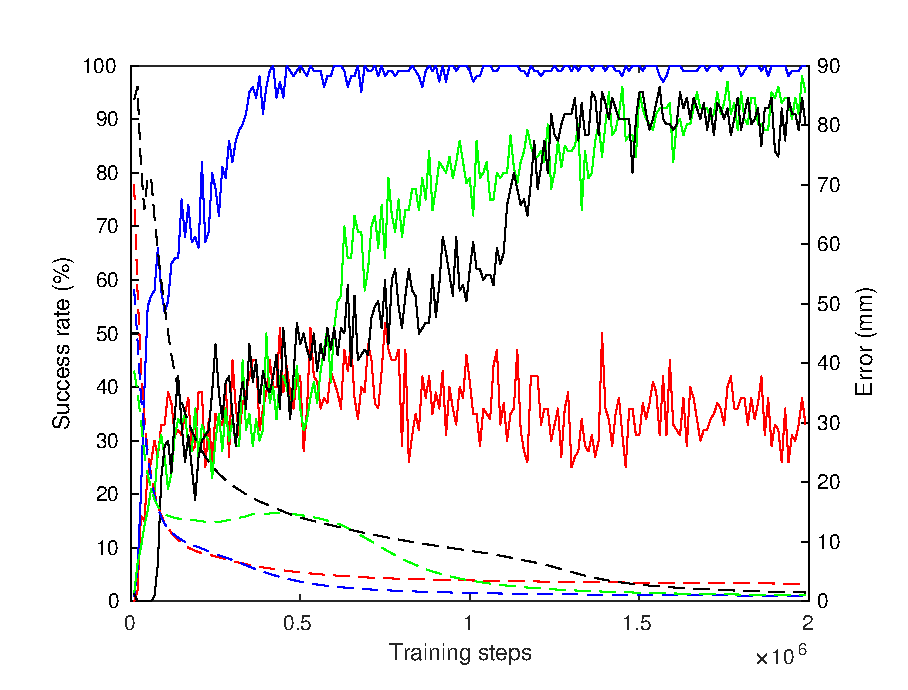
\includegraphics[width=0.33\linewidth]{2-tube-learning.eps}}}
    \subfloat[3 tube]{{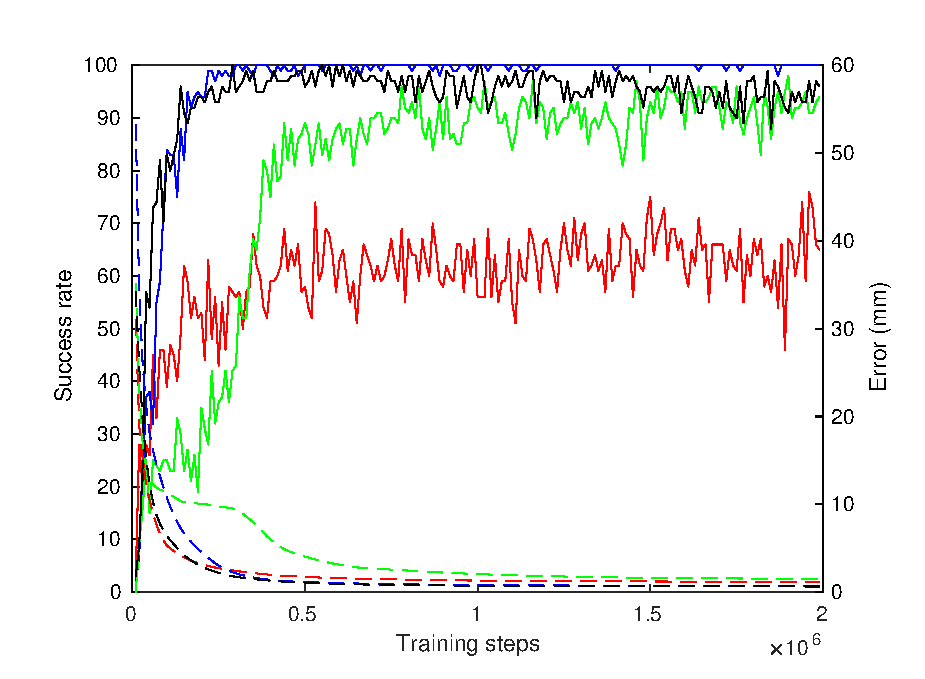
\includegraphics[width=0.33\linewidth]{3-tube-learning.eps}}}
    \subfloat[4 tube]{{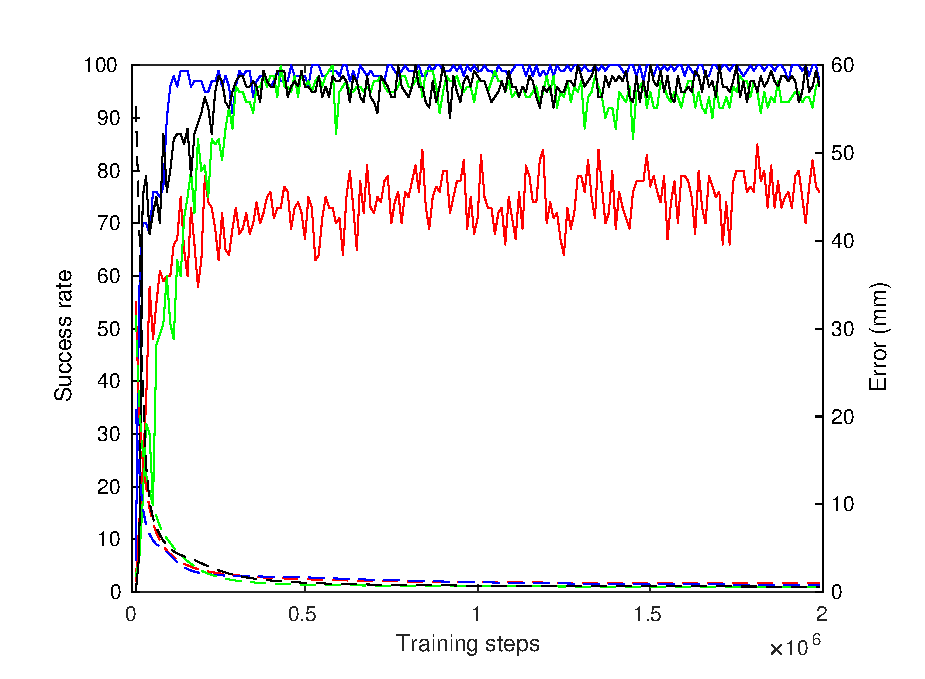
\includegraphics[width=0.33\linewidth]{4-tube-learning.eps}}}
    \caption{Success rate and evaluation error at training episodes. Solid lines are success rate and dashed lines are error. Red is type 1, blue type 2, green type 3 and black type 4.}
    \label{fig:learning-curves}
\end{figure}

\begin{figure}
    \subfloat[2 tube]{{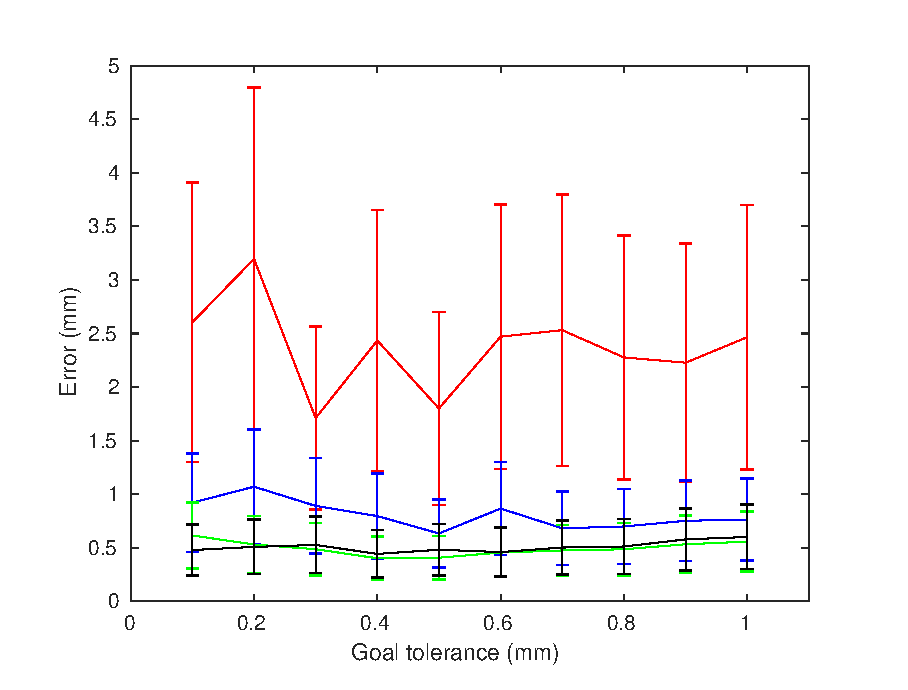
\includegraphics[width=0.33\linewidth]{2-tube-eval.eps}}}
    \subfloat[3 tube]{{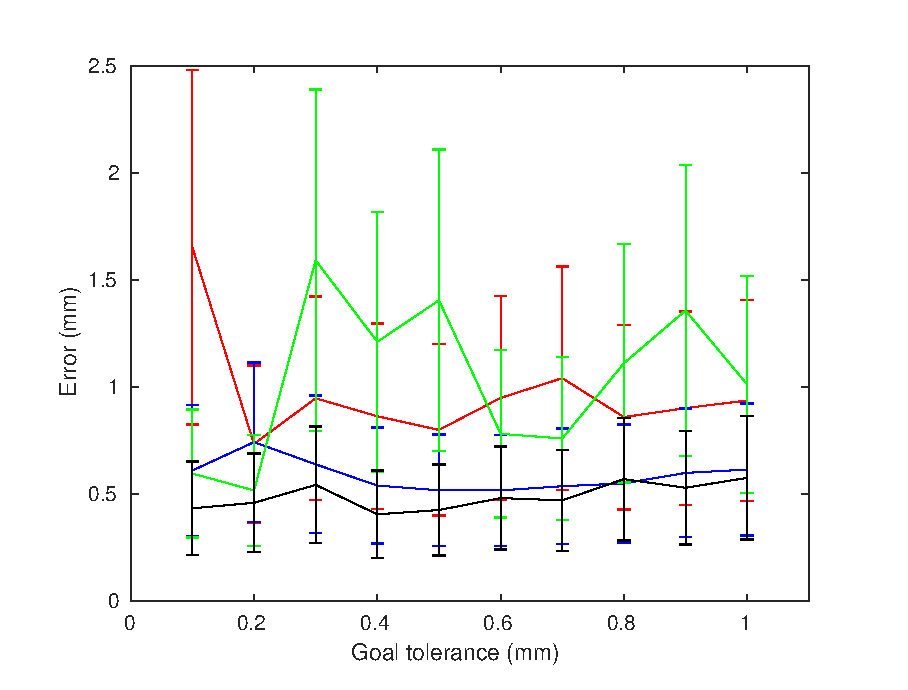
\includegraphics[width=0.33\linewidth]{3-tube-eval.eps}}}
    \subfloat[4 tube]{{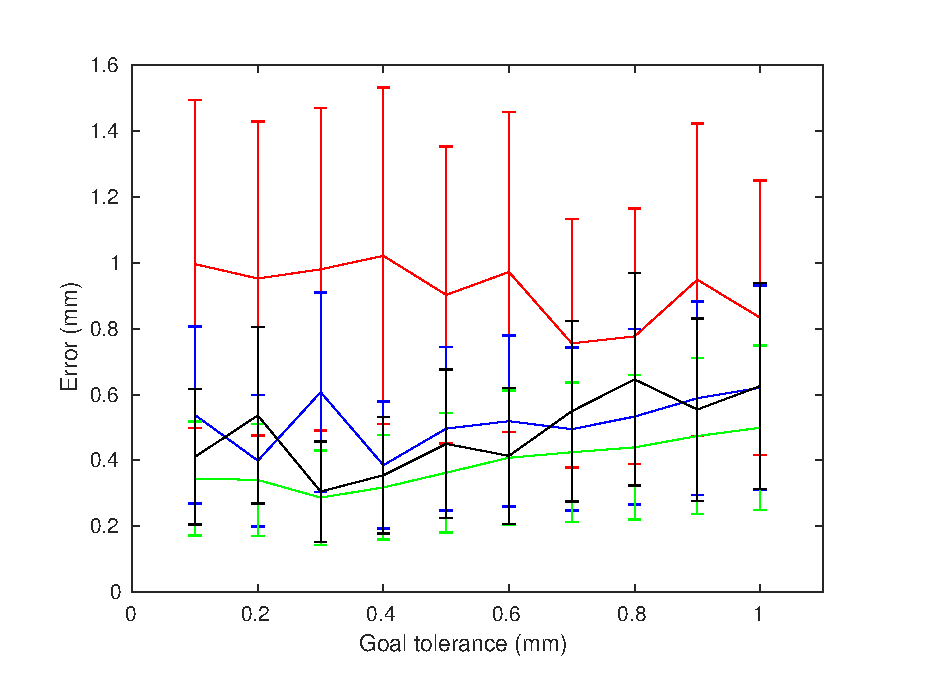
\includegraphics[width=0.33\linewidth]{4-tube-eval.eps}}}
    \caption{Goal tolerance and resulting mean and standard deviation evaluation error. Red is type 1, blue type 2, green type 3 and black type 4.}
    \label{fig:learning-eval}
\end{figure}

For each environment, there are four experiments for each noise type for a total of 12 experiments. The noise type are labelled as  type 1: zero mean multivariate Gaussian noise with a single standard deviation, type 2: zero mean multivariate Gaussian noise with multiple standard deviations, type 3: Ornstein Uhlenbeck noise and type 4: parameter noise. The noise type parameters were found through a hyperparameter search detailed in the previous section and summarized in Table \ref{tab:hyperparam-summary}. Training is done over 2 million timesteps and the results are illustrated in Figure \ref{fig:learning-eval}. Type 1 performs the worst in every environment. It has the lowest success rate and highest evaluation error. This result is expected because having a single noise value for both extension and rotation joints will not explore the Cartesian space correctly. The output of the noise will almost always result in a full extension action or retraction action. This is shown in Figure \ref{fig:two-tube-pcl} where type 1 and type 4 training points are plotted for a two tube environment. The color mapping indicates the Q-value or estimated future cumulative reward at the point. In the type 1 point cloud, the Q-value is uniform with changes in full extension and retraction, joint states visited quite often because of the coarse noise of type 1. This is confirmed with the sparse points on the edges of the workspace. In the type 4 point cloud, the Q-values are mapped with high values in he centre of workspace and lower values at extension. This makes intuitive sense as in general, workspace edge points take more timesteps to achieve, resulting in lower rewards. The points on the edges of the workspace also dense, suggesting these areas are explored during training.

Another result is type 2 converges the fastest and performing the best in evaluation during training. Separating noise for rotation and extension greatly improves overall training performance. The other types, type 3 and type 4, perform moderately in training evaluation converging to a high success rate and low errors nearing the end of 2 million steps. The last result is that the exploration types are scalable with number of tubes. With more tubes, the model convergence of all types improves. We deduce this could be for two reasons. The first is with more tubes, joint redundancy increases. A desired goal can have more that one joint solution, allowing for faster convergence with exploration. Secondly, because of the Cartesian sampling bias, full extension and retraction Cartesian points are sampled less, where redundant joint solutions fewer, making successful episodes more common.
\begin{figure}
    \subfloat[Type 1]{{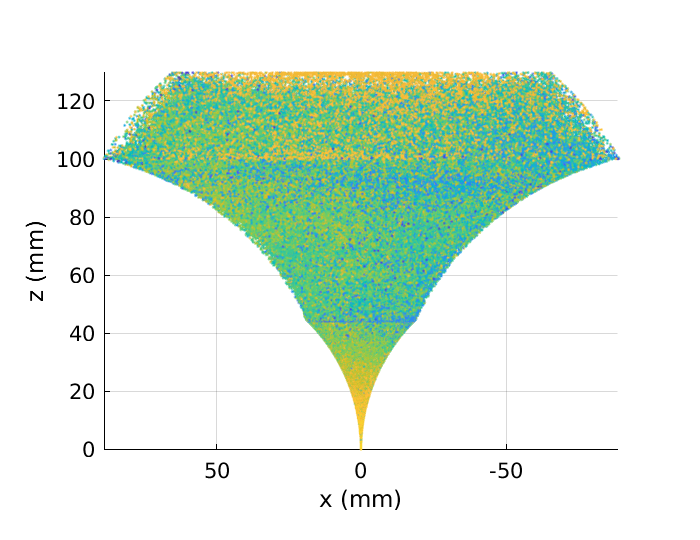
\includegraphics[width=0.5\linewidth]{exp-1-q-values.eps}}}
    \subfloat[Type 4]{{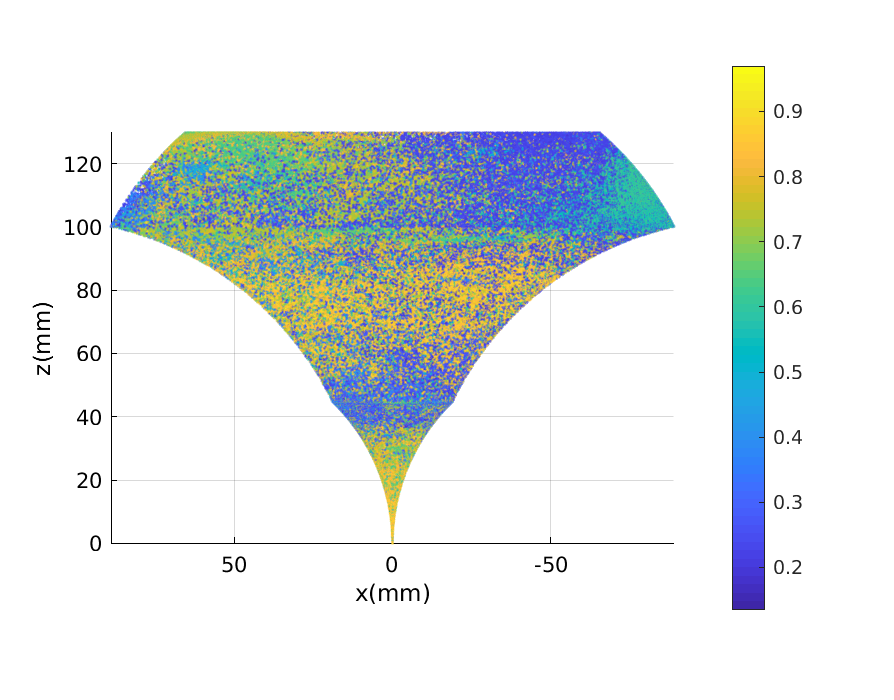
\includegraphics[width=0.5\linewidth]{exp-5-q-values.eps}}}
    \caption{Two tube environment with parameter noise type and 0.6 mm goal tolerance. RGB Q-values are normalzed between 0 and 1 and visualized.}
    \label{fig:two-tube-pcl}
\end{figure}

During training, an error tolerance of 1 mm was set for all experiments. This limits the accuracy of the inverse kinematics, as once an error of just below 1 mm is reached, the episode is terminated, even if the learned policy could move closer with a lower error threshold. To this end, we test lowering the goal tolerance and resulting error in evaluation. Each noise type learned model was evaluated over 5000 timesteps and the overall mean error and standard deviation of error was recorded and illustrated by Figure \ref{fig:learning-eval}. From the plots, its clear that type 3 and type 4 perform better than type one and type two. The error decreases until the 0.1 mm tolerance where an increase can be found in some cases. This represents a key trade-off. As the goal tolerance decreases, success rate and episode length increase. In other words, with lower tolerances more iterations are needed get to the desired goal. This is a parallel to traditional iterative Jacobian where if the do converge to a solution, further iteration can yield higher accuracy with the cost of computation time.

One of the initial problems proposed in this work was exploration due to Cartesian sampling bias and the exploration exploitation trade-off. To demonstrate performance of the noise types in extended states, the last test performed was to test trajectory following a square at extension where Cartesian sampling is low. The trajectory generator would output a point approximately at 100 Hz for 20,000 steps. The reinforcement learning controller received the point and appends the desired goal in the state. While this update is occurring, the controller is iterated through episodes with the learned policy model. We plot the desired and achieved trajectories and errors for two, three and four tube with the best performing noise type, and goal tolerance for each.

\begin{figure}
    \subfloat[Trajectory]{{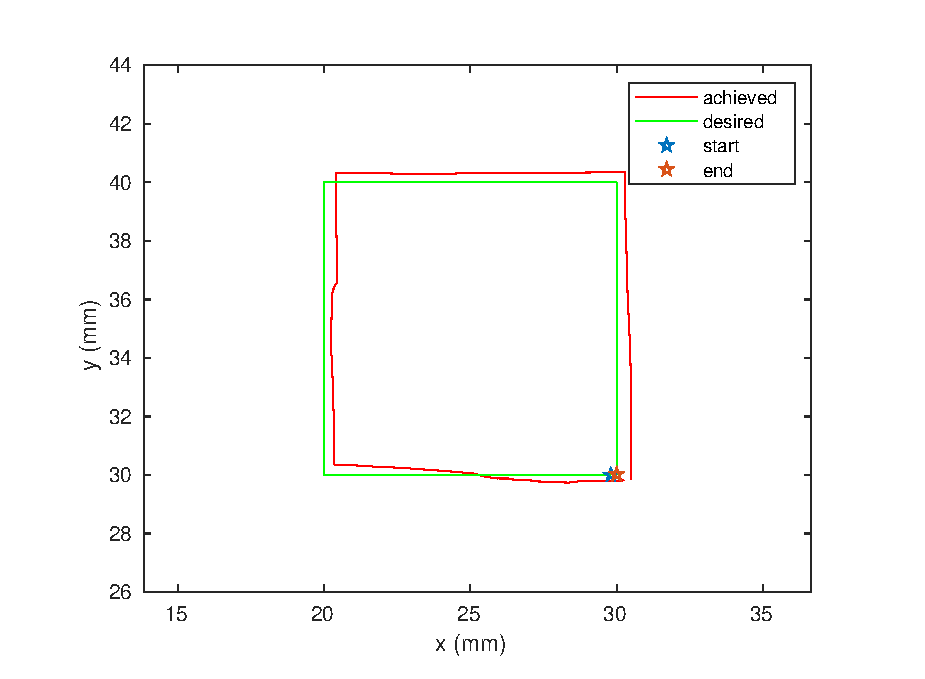
\includegraphics[width=0.5\linewidth]{exp4-square-0-6.eps}}}
    \subfloat[Error]{{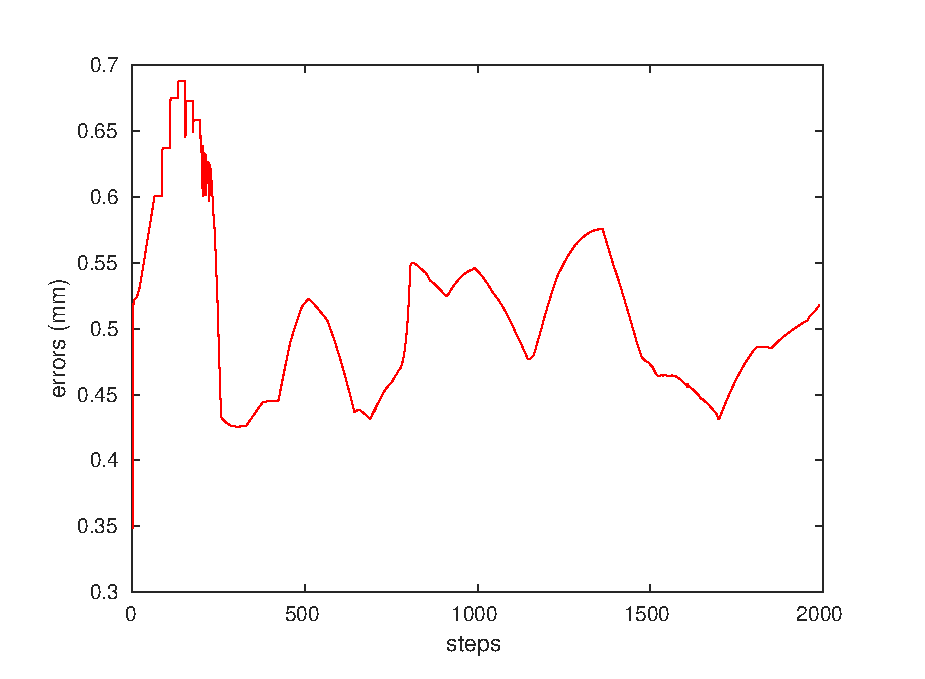
\includegraphics[width=6cm]{exp4-square-0-6-error.eps}}}
    \caption{Two tube environment with type 3 and 0.6 mm goal tolerance.}
    \label{fig:two-tube-traj}
\end{figure}
\begin{figure}
    \subfloat[Trajectory]{{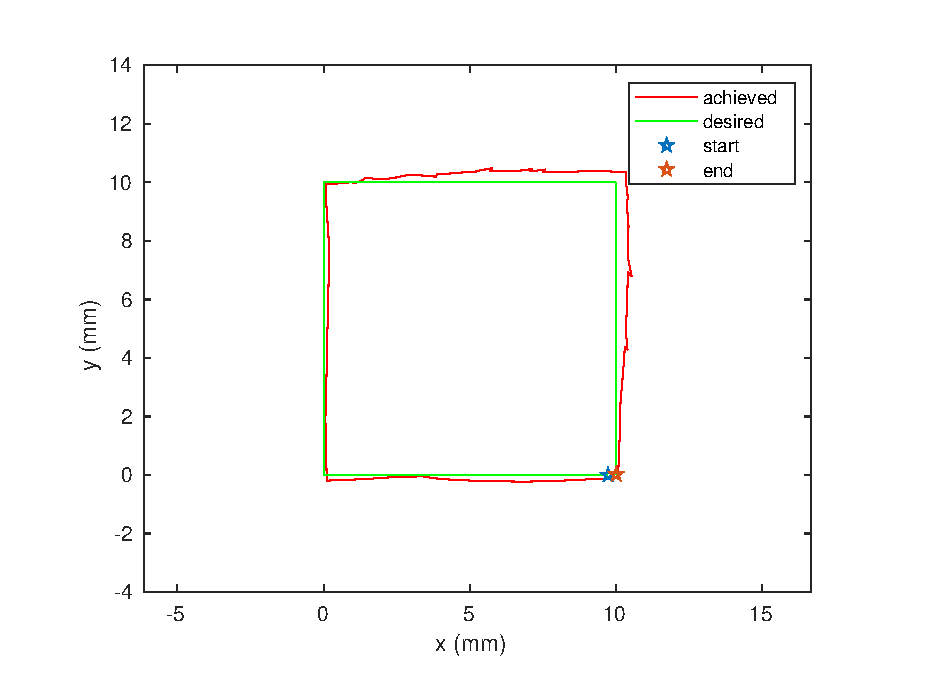
\includegraphics[width=0.5\linewidth]{exp10-square-0-4.eps}}}
    \subfloat[Error]{{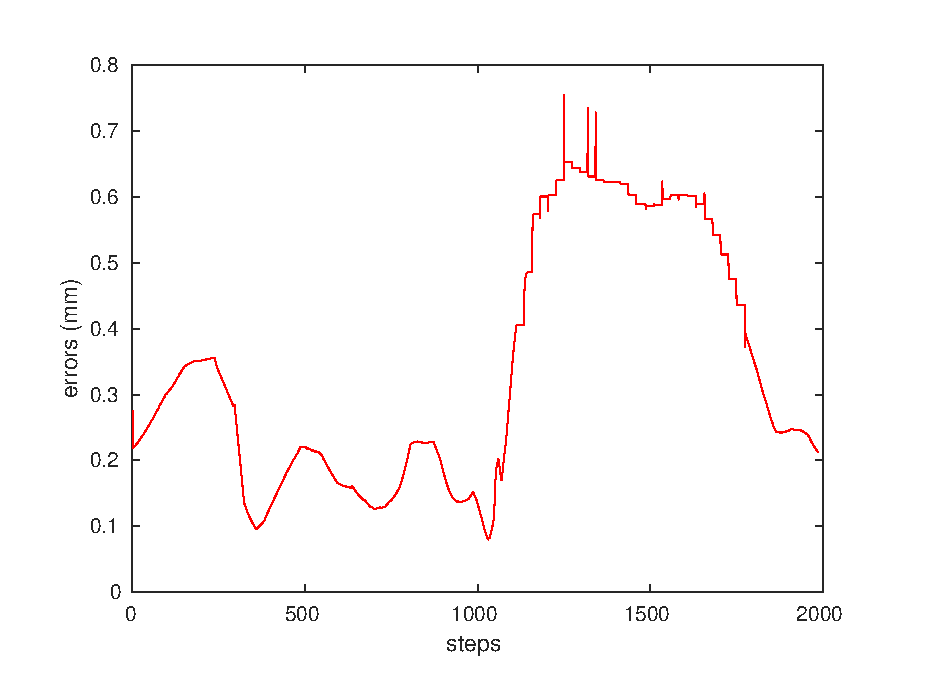
\includegraphics[width=0.5\linewidth]{exp10-square-0-4-error.eps}}}
    \caption{Three tube environment with type 3 and 0.4 mm goal tolerance.}
    \label{fig:three-tube-traj}
\end{figure}
\begin{figure}
    \subfloat[Trajectory]{{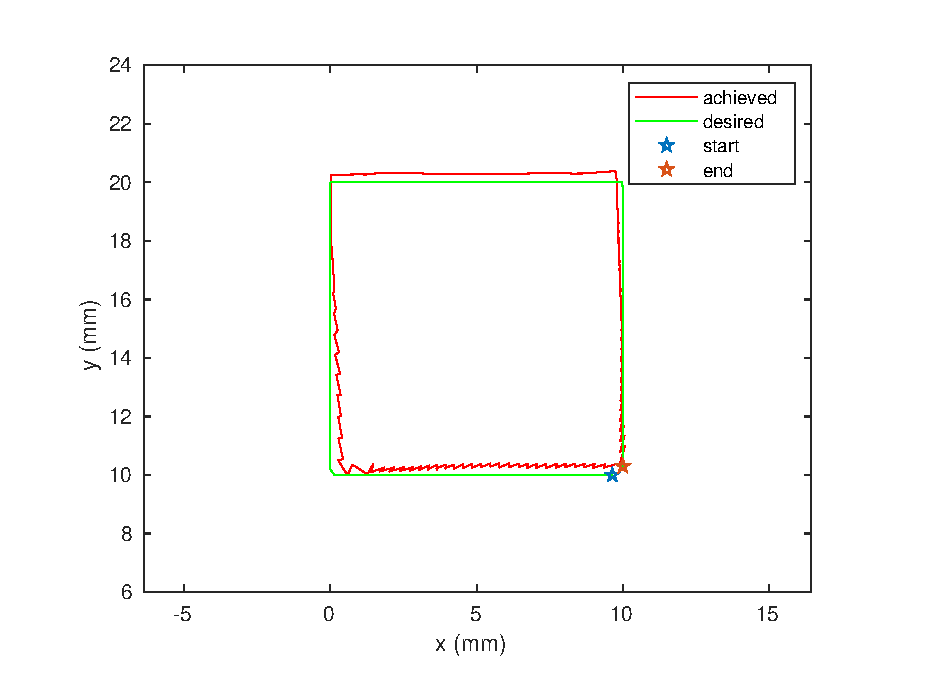
\includegraphics[width=0.5\linewidth]{exp14-square-0-3.eps}}}
    \subfloat[Error]{{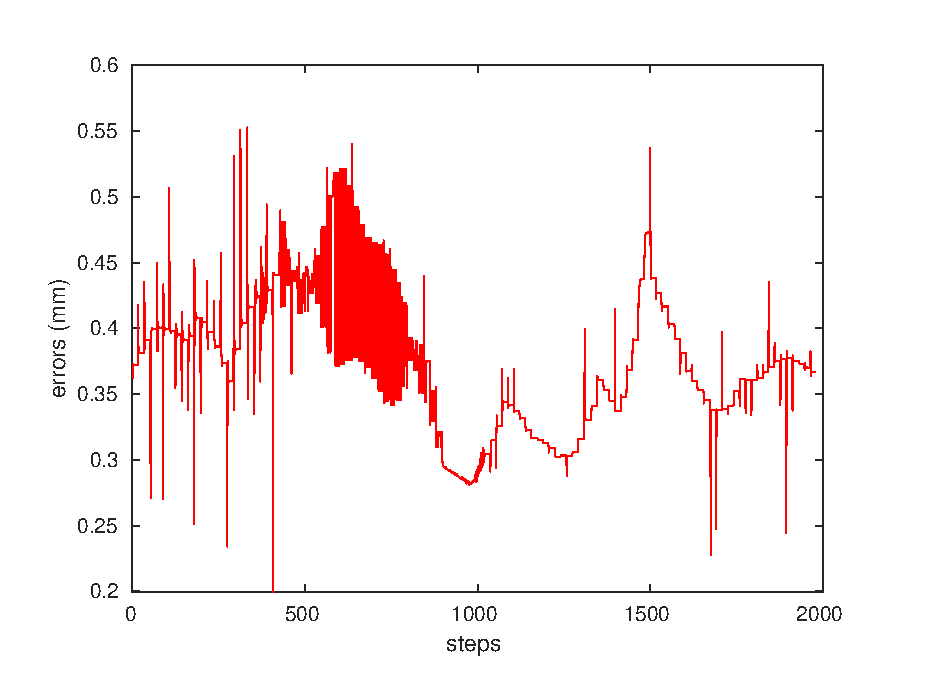
\includegraphics[width=0.5\linewidth]{exp14-square-0-3-error.eps}}}
    \caption{Four tube environment with type 4 and 0.3 mm goal tolerance.}
    \label{fig:four-tube-traj}
\end{figure}

In Figure \ref{fig:two-tube-traj}, a maximum error of 0.70 mm. In the trajectory plot, there seems to be a constant offset in all tests, possibly due to the goal tolerance set. The error plots suggests a similar hypothesis as errors lie above the goal tolerances. In Figure \ref{fig:three-tube-traj}, the error is below 0.4 mm until the third turn where it grows to 0.7 mm but able to reduce to 0.25 mm before the end of the trajectory. In \ref{fig:four-tube-traj}, the errors are similar but the agent is making large action changes in short timesteps causing the errors to oscillate quickly. This behaviour emerges with number of tubes as in Figure \ref{fig:two-tube-traj} no oscillations are found and in Figure \ref{fig:three-tube-traj}, oscillations begin to emerge. Our hypothesis for this behaviour has to do with joint redundancy. With more tubes, a single desired goal can have multiple solutions and when the agent is selecting actions, a small change in the state from a previously selected action can result in a completely different next action. These issues parallel iterative methods and pre-computing trajectories offline can greatly improve oscillations and errors in general.


\section{Conclusion and Future Work}
In this work, the different noise types used for model-free deep reinforcement learning were studied in the context of concentric tube robots. Sampling bias and joints with different units of actuation make exploration a challenge, an important factor in reinforcement learning convergence. A single standard deviation zero mean multivariate Gaussian noise process performed the worst, with low success rates and high error. A multi-standard deviation multivariate zero mean Gaussian noise process, where rotation and extension action standard deviation were separated in the co-variance matrix performed best during training. When the goal tolerance was changed, parameter noise was found to perform better in evaluation with smaller goal tolerances. Using the best noise type model and goal tolerance for each environment, a test to follow a square trajectory at extension was done. Sampling high extension values is low, so high extension was chosen for the plane of the square. The results show an online trajectory controller using reinforcement learning for concentric tube robots can follow a square trajectory with less than 0.7 mm for 2 tubes and less than 0.5 mm for 4 tube.

A large caveat is the use of the dominant stiffness model. Future work should use a torsionally compliant variable stiffness model and stability conditions for training using the parameter noise type. 
%\begin{acknowledgements}
%If you'd like to thank anyone, place your comments here
%and remove the percent signs.
%\end{acknowledgements}


% Authors must disclose all relationships or interests that 
% could have direct or potential influence or impart bias on 
% the work: 
%
\section*{Conflict of interest}
The authors Keshav Iyengar, George Dwyer and Danail Stoyanov, confirm that they do not have financial or non-financial conflict of interest related to the work presented in this paper and that the research here detailed did not involve human participants or animals, hence, the need for informed consent does not apply.
%
% The authors declare that they have no conflict of interest.


% BibTeX users please use one of
%\bibliographystyle{spbasic}      % basic style, author-year citations
\bibliographystyle{spmpsci}      % mathematics and physical sciences
%\bibliographystyle{spphys}       % APS-like style for physics
\bibliography{refs}   % name your BibTeX data base

% Non-BibTeX users please use
%\begin{thebibliography}{}
%
% and use \bibitem to create references. Consult the Instructions
% for authors for reference list style.
%
% \bibitem{RefJ}
% Format for Journal Reference
% Author, Article title, Journal, Volume, page numbers (year)
% Format for books
% \bibitem{RefB}
% Author, Book title, page numbers. Publisher, place (year)
% etc
% \end{thebibliography}

\end{document}
% end of file template.tex

